\documentclass{article}

\usepackage[top=1in,bottom=0.5in,left=0.5in,right=0.5in]{geometry}
\usepackage{amsmath,amssymb,multirow,graphicx}

\newcommand{\bx}{\mathbf{x}}
\newcommand{\by}{\mathbf{y}}
\newcommand{\bn}{\mathbf{n}}
\newcommand{\bu}{\mathbf{u}}

\begin{document}
\section*{Table of Quadrature Results for Regularized Stokeslets}

We are solving for the fluid flow around a steadily translating cylinder of radius $a=0.25$ in an infinite fluid with viscosity $\mu=1.0$. We use the 2D steady Stokes equations $\mu\Delta \bu(\bx) = -\nabla p$ with boundary conditions $\bu = [1,0]$ on the circle to approximate the solution near the cylinder. See Cortez (2001) for more details and the formula for the exact solution to the test case. We use a regularization method on the kernel of the integral equation combined with various boundary element methods (BEMs) to solve the problem numerically.

Table 1 lists the errors for a single point slightly outside of the cylinder: $0.26*(\cos(\pi/6),\sin(\pi/6))$. We discretize the boundary circle into $N$ nodes and represent the circle as an $N$-polygon. The numerical methods examined are the original method by Cortez (2001) (called ``Riemann Sum'' in the table), and either hat, constant, or blob basis functions paired with either the trapezoidal rule or Simpson's rule for numerical integration along each chord comprising the polygon. Quadrature is performed with $M$ points along each chord. In Table 1, $M=1000$ excluding the ``Riemann Sum'' column, where $M=1$ to be equivalent with the original model. Each chord is length $\ell = 2\sin(\pi/N)$, and the quadrature spacing is $\ell/M$. The blob parameter for the regularization is $\ell/4$ in all trials in Table 1, so it is decreasing as chord length decreases.


\begin{table}[h]
	\begin{centering}
\begin{tabular}{|c|c|c|c|c|c|c|c|}
	\hline
	$N$ & Riemann Sum & Blob, Trap & Blob, Simp & Hat, Trap & Hat, Simp & Cst, Trap & Cst, Simp  \\
	\hline
	   4 & 2.5103  &  0.0435  &  0.0435  &  0.0516  &  0.0516  &  4.2663  &  4.2664		\\
	   8 & 0.0280  &  0.0130  &  0.0130  &  0.0065  &  0.0065  &  0.0099  &  0.0099     \\
	  16 & 0.0189  &  0.0117  &  0.0117  &  0.0071  &  0.0071  &  0.0072  &  0.0072     \\
	  32 & 0.0097  &  0.0072  &  0.0072  &  0.0055  &  0.0055  &  0.0055  &  0.0055     \\
	  64 & 0.0049  &  0.0037  &  0.0037  &  0.0035  &  0.0035  &  0.0035  &  0.0035     \\
	 128 & 0.0024  &  0.0020  &  0.0020  &  0.0019  &  0.0019  &  0.0019  &  0.0019     \\
\hline
	$N$ & Err/$\ell$ & Err/$\ell$ & Err/$\ell$ & Err/$\ell$ & Err/$\ell$ & Err/$\ell$ & Err/$\ell$  \\
\hline  
 4 & 1.7750e+00 & 3.0794e-02 & 3.0794e-02 & 3.6498e-02 & 3.6498e-02 & 3.0168e+00 & 3.0168e+00 \\
   8 & 3.6605e-02 & 1.6934e-02 & 1.6934e-02 & 8.5116e-03 & 8.5116e-03 & 1.2994e-02 & 1.2994e-02 \\
  16 & 4.8429e-02 & 3.0111e-02 & 3.0111e-02 & 1.8181e-02 & 1.8181e-02 & 1.8330e-02 & 1.8330e-02 \\
  32 & 4.9702e-02 & 3.6751e-02 & 3.6751e-02 & 2.8035e-02 & 2.8035e-02 & 2.8027e-02 & 2.8027e-02 \\
  64 & 5.0054e-02 & 3.7845e-02 & 3.7845e-02 & 3.5383e-02 & 3.5383e-02 & 3.5377e-02 & 3.5377e-02 \\
 128 & 4.7881e-02 & 4.0232e-02 & 4.0232e-02 & 3.8575e-02 & 3.8575e-02 & 3.8575e-02 & 3.8575e-02 \\
\hline
\end{tabular}
\caption{Errors in BEM on the regularized Stokes cylinder example using $N$ chords. The ``Riemann Sum'' column corresponds to the original method introduced by Coretz (2001). the other trials are boundary element methods using either hat or constant functions as a basis and using either the trapezoid rule or Simpson's rule to do quadrature over each chord with 1000 points per chord. The values in the upper half of the table are the errors for the point $0.26*(\cos(\pi/6),\sin(\pi/6))$. The values in the lower half of the table are the errors normalized by the chord length.}
\end{centering}
\end{table}

There are three things to note about Table 1. First, it can be seen that it doesn't matter very much which BEM is used with the regularization. In fact, even the original method has comparable accuracy for $N=128$, implying that using $1000$ quadrature points is major over-kill. Second, all the methods are approximately $O(\ell)$, as seen from the lower half of the table, regardless of numerical integration method. Higher order integration methods might allow us to use fewer points per chord to achieve the same level of accuracy, but -- as will be seen below -- even with only $10$ integration points per chord reasonable accuracy can be achieved with the trapezoid rule. Last, using the blob function itself as a basis does not give very good accuracy, even though in some sense it is a natural choice. This is maybe because it is not exactly $0$ outside of a single element. 

Smith (2009) claims that using a BEM 1) allows the use of fewer points to get comparable accuracy, and 2) weakens the coupling between the blob parameter $\epsilon$ and the discretization mesh parameter choices. The first claim appears to be supported by Table 1, although to truly save computation time, a smaller number of integration points should be used. However, I am not sure that the second claim has much impact. I found that the blob parameter is strongly coupled to the number of chords chosen, $N$ (effectively the discretization of the forces around the boundary), but is maybe decoupled from the number of integration points per chord, $M$. I did a log 10 space exploration of 100 blob parameters from 1.5e-4 to 3.0e-2 and found error minima for $N = 8,\,16,\,32,\,64,\,128,\,256$. These calculations all used hat basis functions and a trapezoid integration rule with $M=10$. None of the minimal errors occurred at the endpoints of the range. The blob parameters associated with these minimal errors are log-log plotted in Figure \ref{bps} against chord length, showing an approximate power law relationship of 3/2. Table 2 gives the blob parameters themselves. 

\begin{table}[ht]
	\begin{centering}
\begin{tabular}{|c|cccccc|}
	\hline
	$N$ &  8 & 16 & 32 & 64 & 128 & 256 \\
	$\ell$ & 7.6537e-01 &  3.9018e-01 &  1.9603e-01  & 9.8135e-02  & 4.9082e-02 &  2.4543e-02  \\
	 ``best''  $\epsilon$ &    2.5550e-02& 5.4120e-03& 1.7590e-03& 7.4709e-04& 3.3476e-04& 1.5825e-04   \\
\hline
\end{tabular}
\caption{For each $N$ and associated chord length $\ell$, $\epsilon$ is the blob parameter resulting in the minimal error on the test case. This minimum is based on a search over 100 values of $\epsilon$ evenly distributed in log-10 space between 1.5e-4 and 3.0e-2, using hat basis functions and the trapezoid rule with $M=10$. }
\end{centering}
\end{table}

\begin{figure}[ht]
\begin{center}
	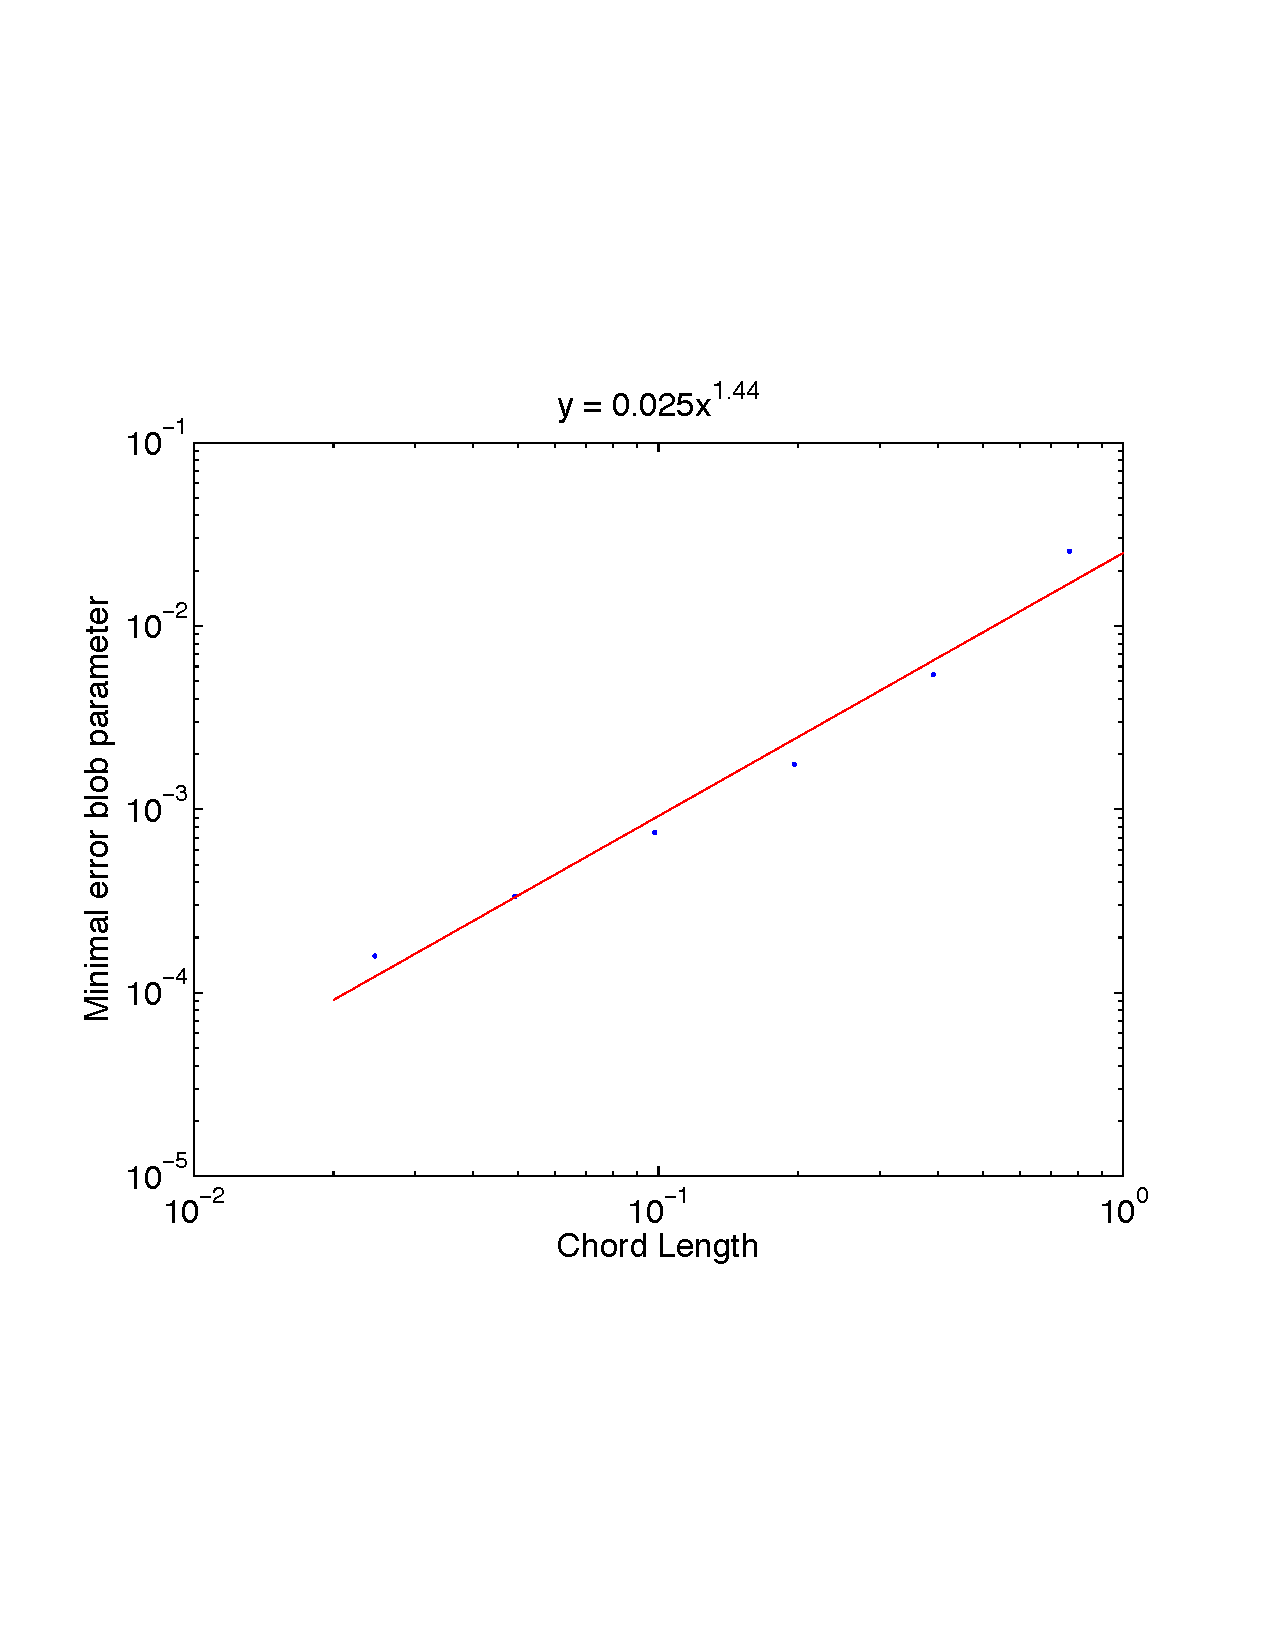
\includegraphics[width=4.0in]{idealblobparam.pdf}
\end{center}
\caption{Log-log plot of the minimal error blob parameter versus chord length (dots). The line is the best fit power law. The dots correspond (from left to right) to $N = 256,\,128,\,64,\,32,\,16,\,8$.}
\label{bps}
\end{figure}	

\pagebreak
For the blob parameters in Table 2, I calculated the error for $M$ varying between 10 and 250 (Table 3). The errors for $N \leq 32$ monotonically decrease with $M$, as one would expect in numerical integration. For higher numbers of chords, the minimal error occurs at $M=20$ and the asymptotic error is higher. I am not sure what to make of this fact, but the differences between $M=20$ and $M>20$ are on order of 1.e-6, so this might be some kind of negligible numerical artifact. 

At this point, I am willing to tentatively agree with Smith (2009) that the number of integration points is not coupled to $\epsilon$. However, the number of chords \emph{is} coupled to $\epsilon$, and both of sets of points comprise the discretization mesh. I suppose he is right in saying that the coupling is weakened, but I am not sure how much we actually gain from this weakening. If the blob parameter corresponds to a physical quantity, then the number of chords should be calculated from the choice of blob parameter, based on some figure like Figure \ref{bps}, and the number of integration points $M$ should be chosen to reduce the integration error to a level below the regularization error. Comparing the Riemann sum errors to the BEM errors in Table 1, it is unclear that we gain that much from this procedure in this example, except at very low chord numbers.



\begin{table}[ht]
	\begin{centering}
\begin{tabular}{|c|c|c|c|c|c|c|c|c|c|}
	\hline
	$N$ & $M=10$ &$M=20$ &$M=30$ &$M=40$ & $M=50$ & $M=100$ &$M=150$& $M=200$ &$M=250$  \\
	\hline
	   8 &  2.0385e-03 &  2.0050e-03 &  1.9990e-03 &  1.9970e-03 &  1.9960e-03 &  1.9947e-03 &    1.9945e-03 &  1.9944e-03 &  1.9943e-03  \\
	  16 &  1.0802e-03 &  8.6211e-04 &  8.5578e-04 &  8.5495e-04 &  8.5461e-04 &  8.5417e-04 &    8.5409e-04 &  8.5406e-04 &  8.5404e-04  \\
	  32 &  5.9662e-04 &  4.0789e-04 &  4.0165e-04 &  4.0086e-04 &  4.0064e-04 &  4.0041e-04 &    4.0037e-04 &  4.0036e-04 &  4.0035e-04  \\
	  64 &  3.5328e-04 &  2.7316e-04 &  2.7381e-04 &  2.7386e-04 &  2.7383e-04 &  2.7378e-04 &    2.7377e-04 &  2.7376e-04 &  2.7376e-04  \\
	 128 &  1.9975e-04 &  1.6297e-04 &  1.6485e-04 &  1.6514e-04 &  1.6517e-04 &  1.6516e-04 &    1.6516e-04 &  1.6516e-04 &  1.6516e-04  \\
	 256 &  1.0707e-04 &  8.7104e-05 &  8.8272e-05 &  8.8477e-05 &  8.8507e-05 &  8.8510e-05 &    8.8509e-05 &  8.8509e-05 &  8.8509e-05  \\
\hline
\end{tabular}
\caption{Errors in BEM on the regularized Stokes cylinder example using hat basis functions with the trapezoid rule. The blob parameter is the same as in Figure \ref{bps} (blue dots). $M$ is the number of integration points per chord; the number of chords is $N$. The values in the table are the errors for the point $0.26*(\cos(\pi/6),\sin(\pi/6))$. }
\end{centering}
\end{table}

Since I have only looked at the error at a single point, further validation is required to make sure that the numerical implementation is working properly. Figure \ref{vel} shows the $u$ and $v$ velocity contours for a numerical solution with hat basis functions, a trapezoidal quadrature rule, $N=256$, $M=20$, and $\epsilon=$1.5825e-04 (black lines). These results are superposed over the exact solution (red lines). Note that the solution is quite poor inside the cylinder, but is robust outside of the cylinder. I do not why this is happening, but the point used in all the experiments above should be fine.

\begin{figure}[ht]
\begin{tabular}{cc}
	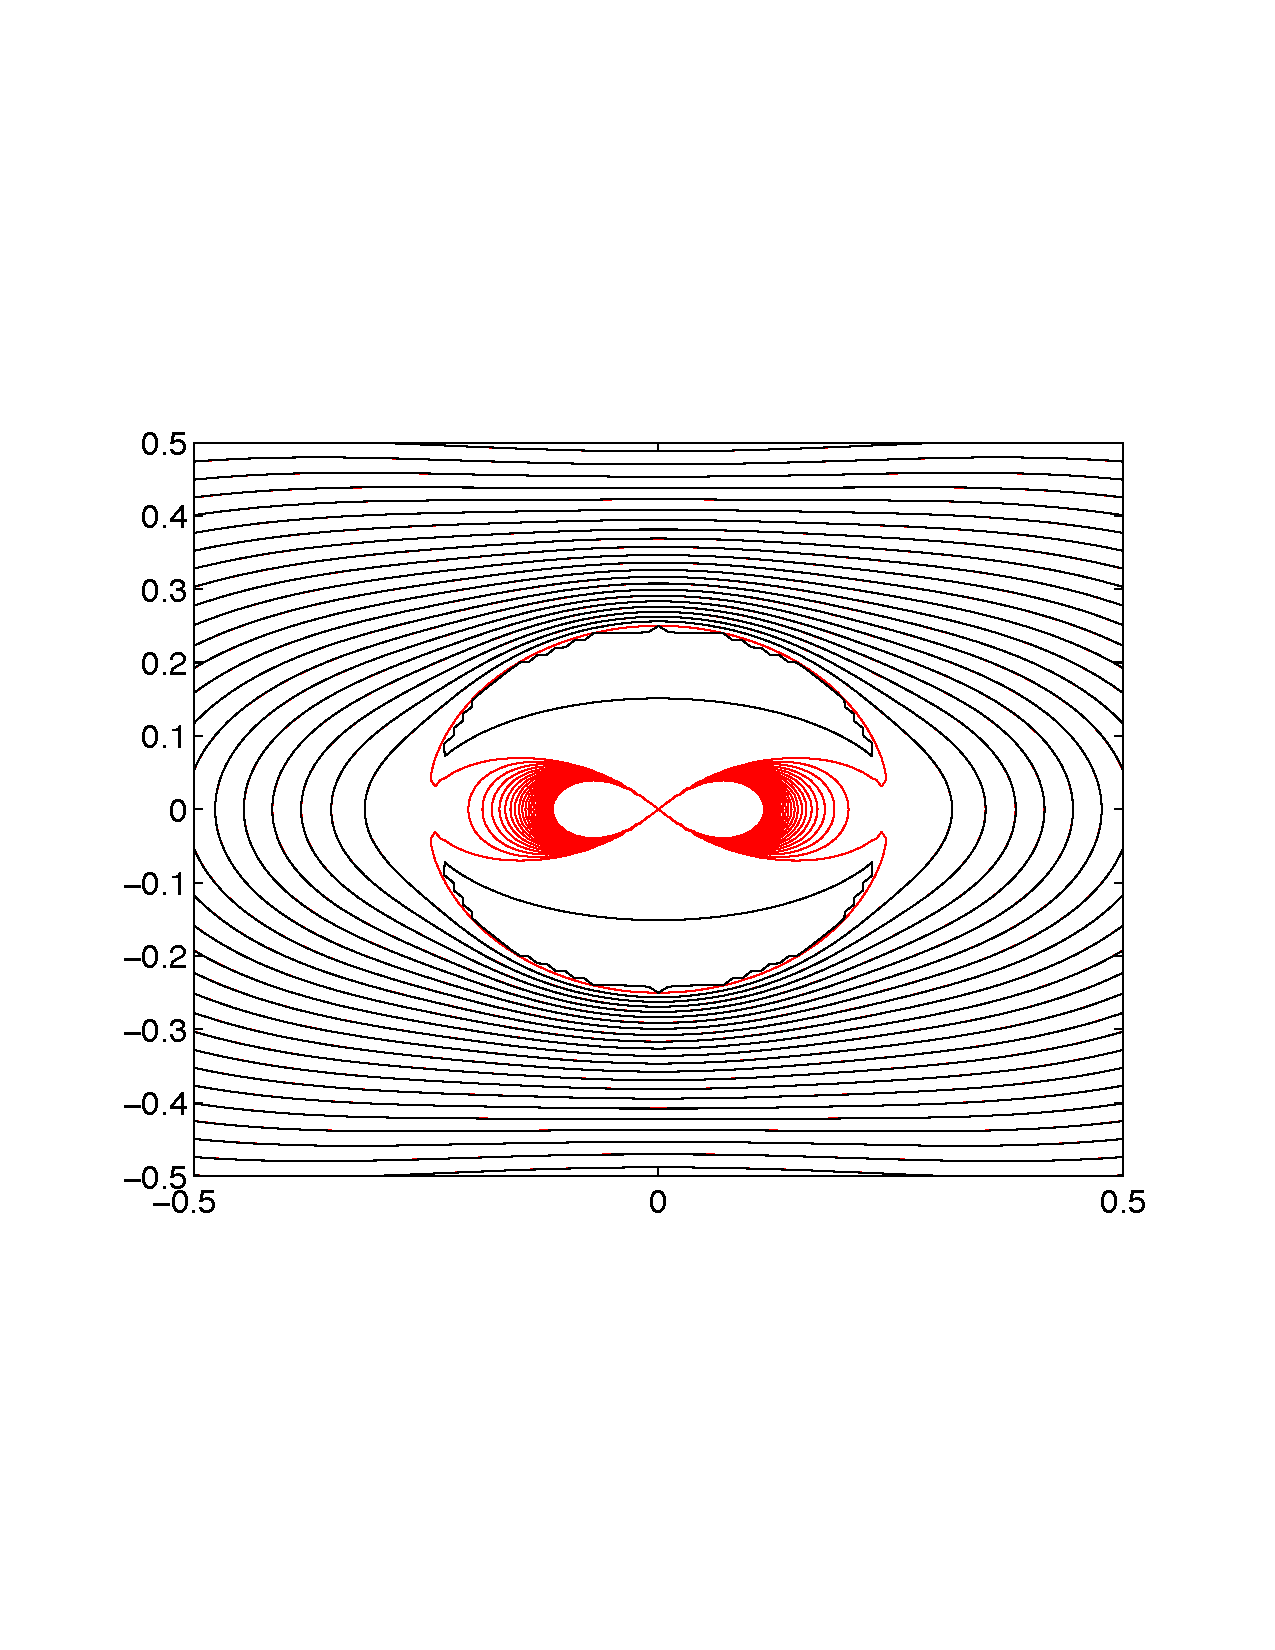
\includegraphics[width=3.25in]{uvel.pdf} & 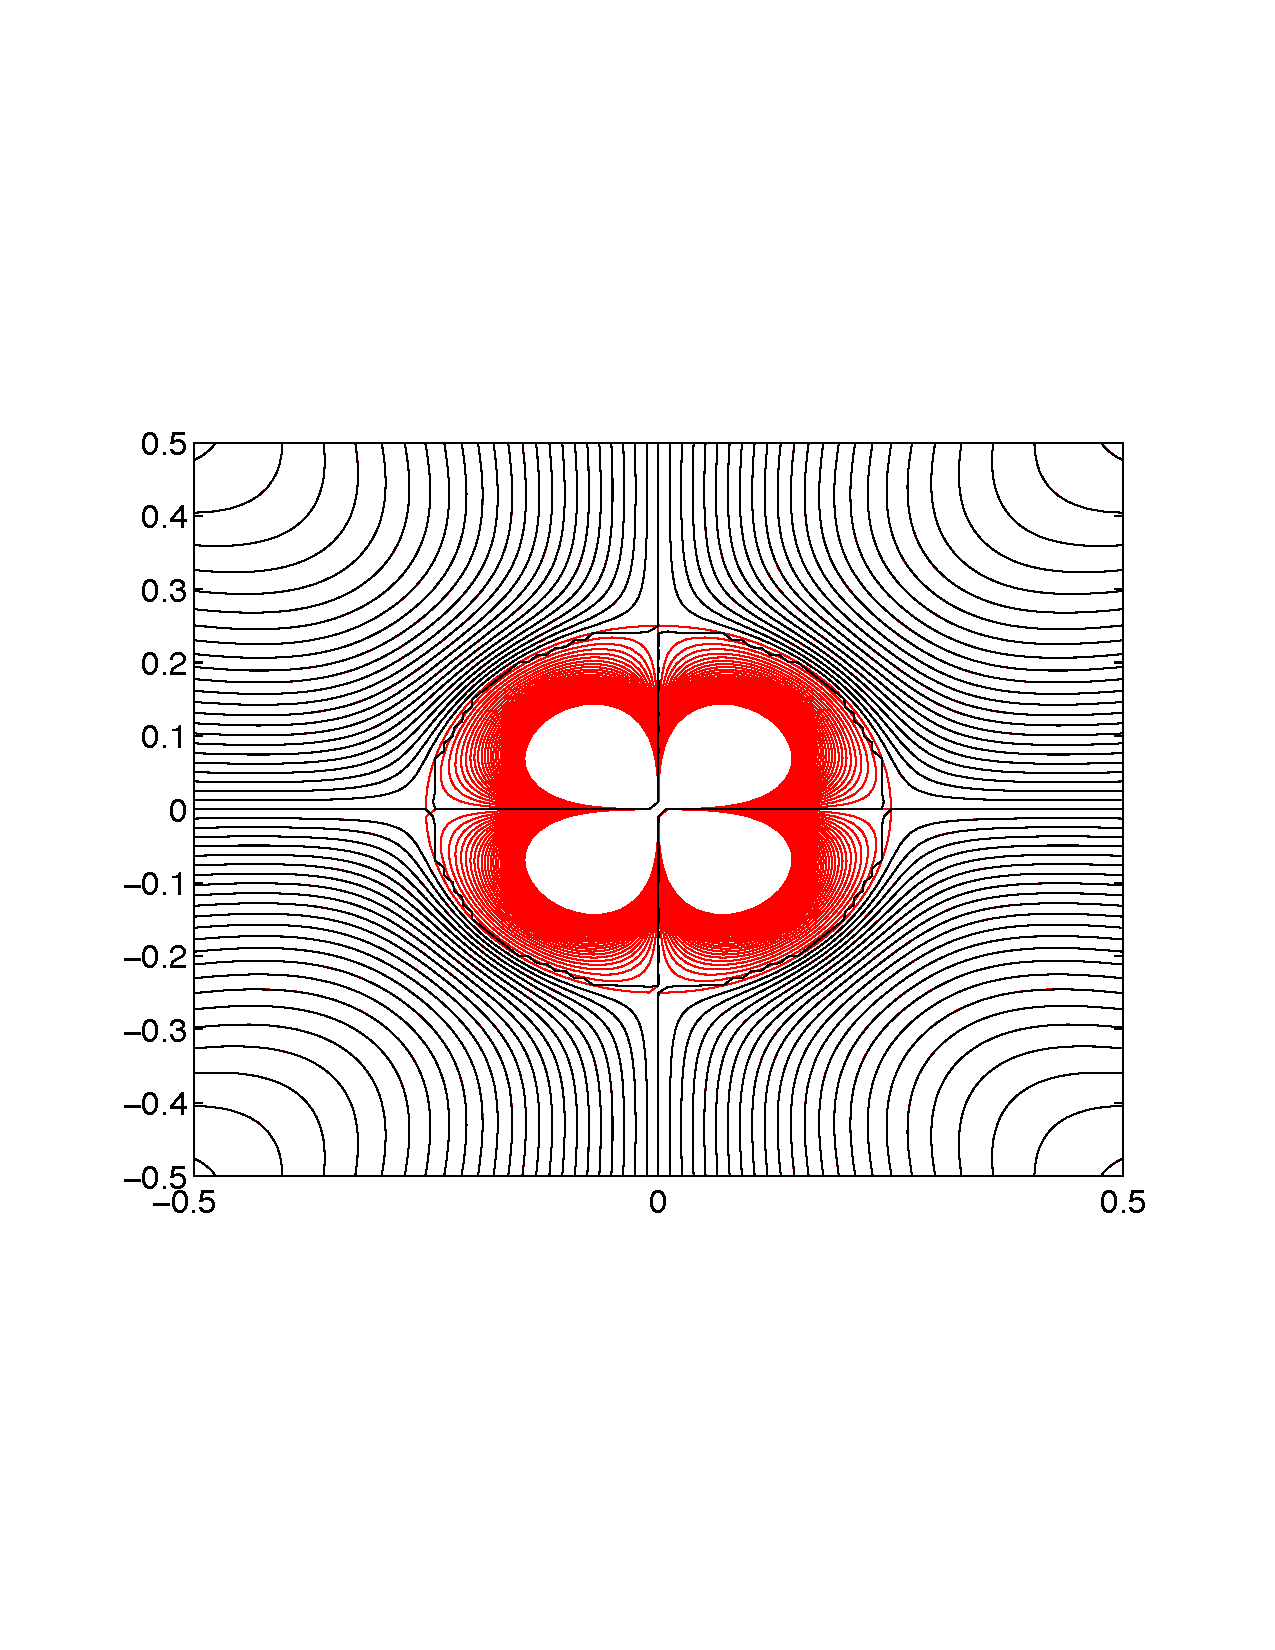
\includegraphics[width=3.25in]{vvel.pdf}\\
	A & B 
\end{tabular}
\caption{A. The contours of the component of velocity in the $x$-direction, $u$, in the square [-0.5, 0.5] x [-0.5, 0.5]. B. The same for the $y$-component, $v$.}
\label{vel}
\end{figure}	

\section*{Blob parameters}

We examine the same problem using the $L_2$ error over square patches of velocity both near and far from the circle as in Fig. \ref{schematic}.

\begin{figure}[ht]
	\begin{center}
	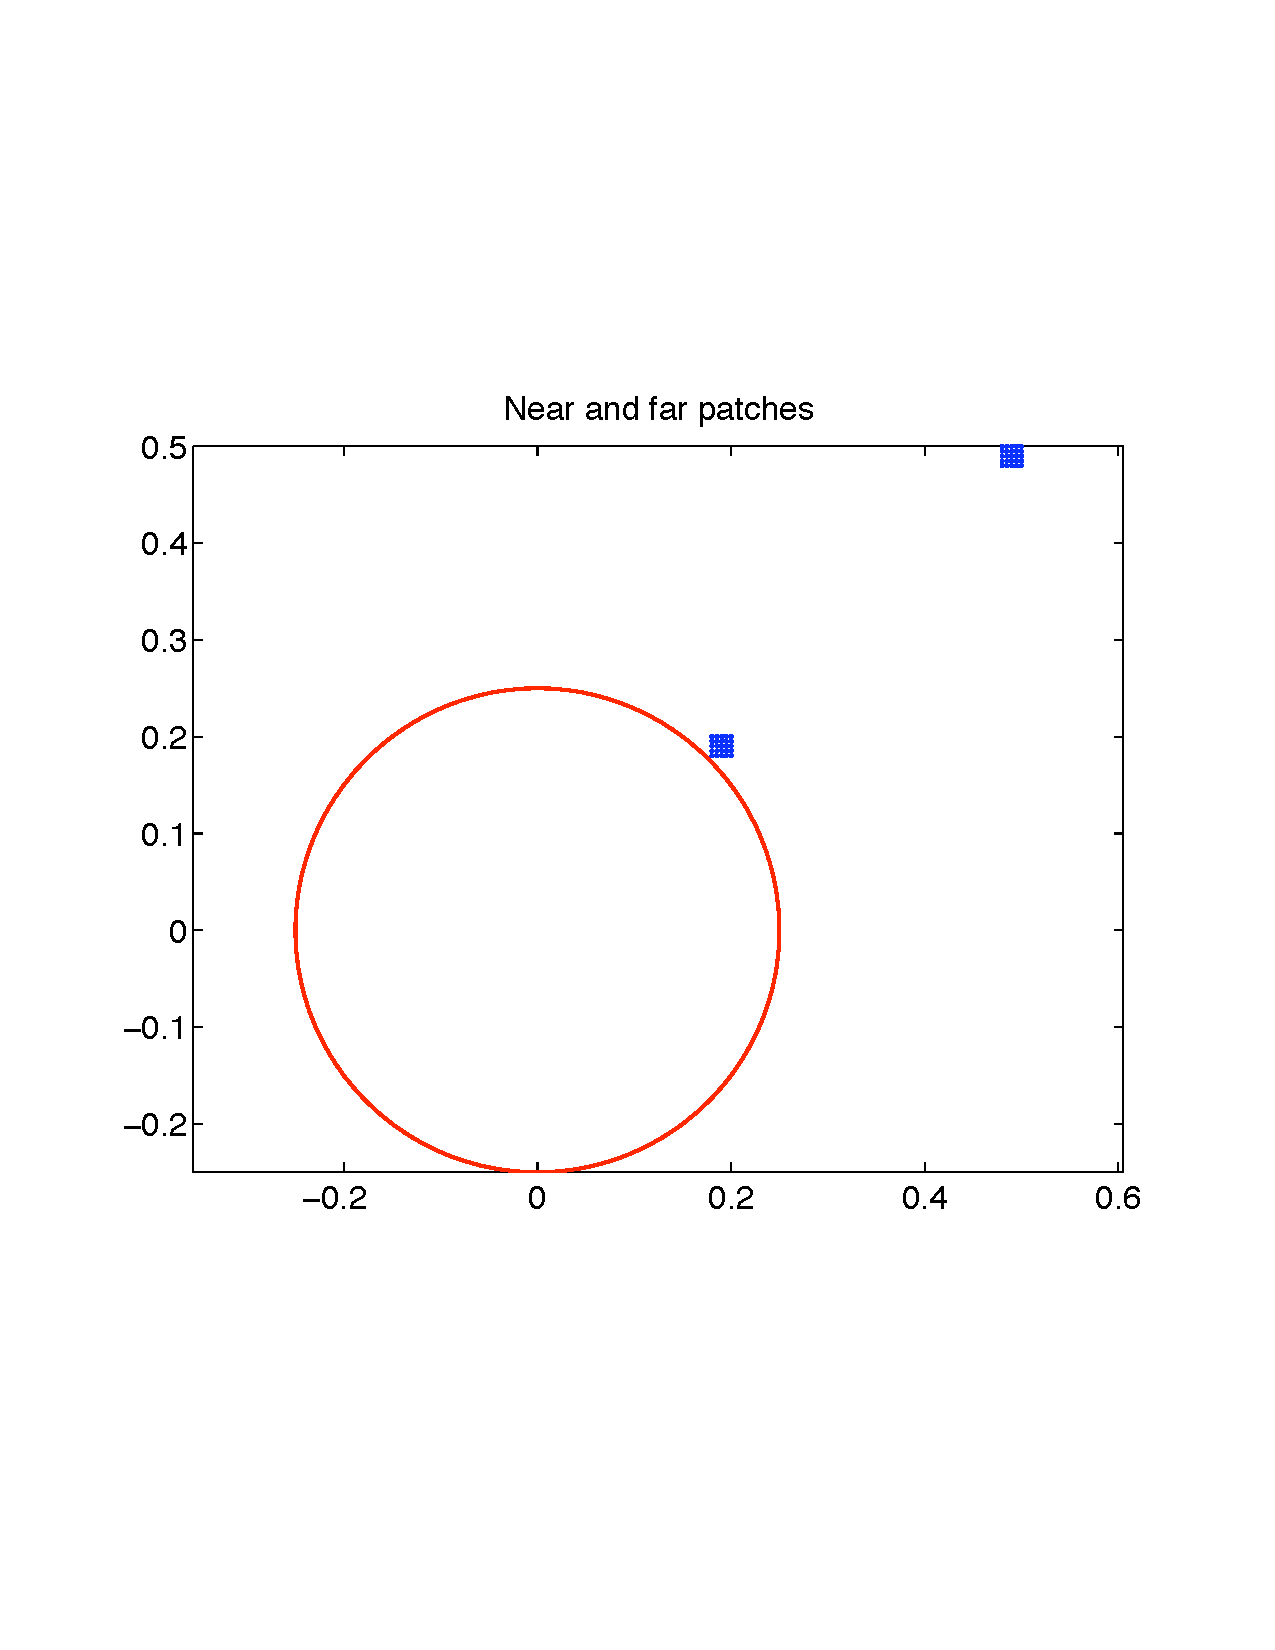
\includegraphics[width=3.0in]{StokesCylTest_farnearpatches_schematic.pdf}
\end{center}
\caption{The near and far patches on which the $L_2$ error is calculated.}
\label{schematic}
\end{figure}	

First we look at the difference between the original method and a BEM with hat basis functions and the trapezoidal rule with 20 points per chord. We plot error versus blob parameter value for differing numbers of chords ($N$) in Fig. \ref{errvsbp}. The original method and the BEM method are very similar for large $N$ or large $\epsilon$, but overall the BEM offers more flexibility in the choice of $\epsilon$ for a given error level.

We then fix blob parameters and plot $L_2$ error versus the number of chords. The results for 4 different blob parameters are in Fig. \ref{errvsN}. For a large enough blob parameter, the results of the original method versus the BEM are the same, but at smaller blob parameters and lower $N$, the BEM has a much lower error.


\begin{figure}[ht]
\begin{tabular}{cc}
	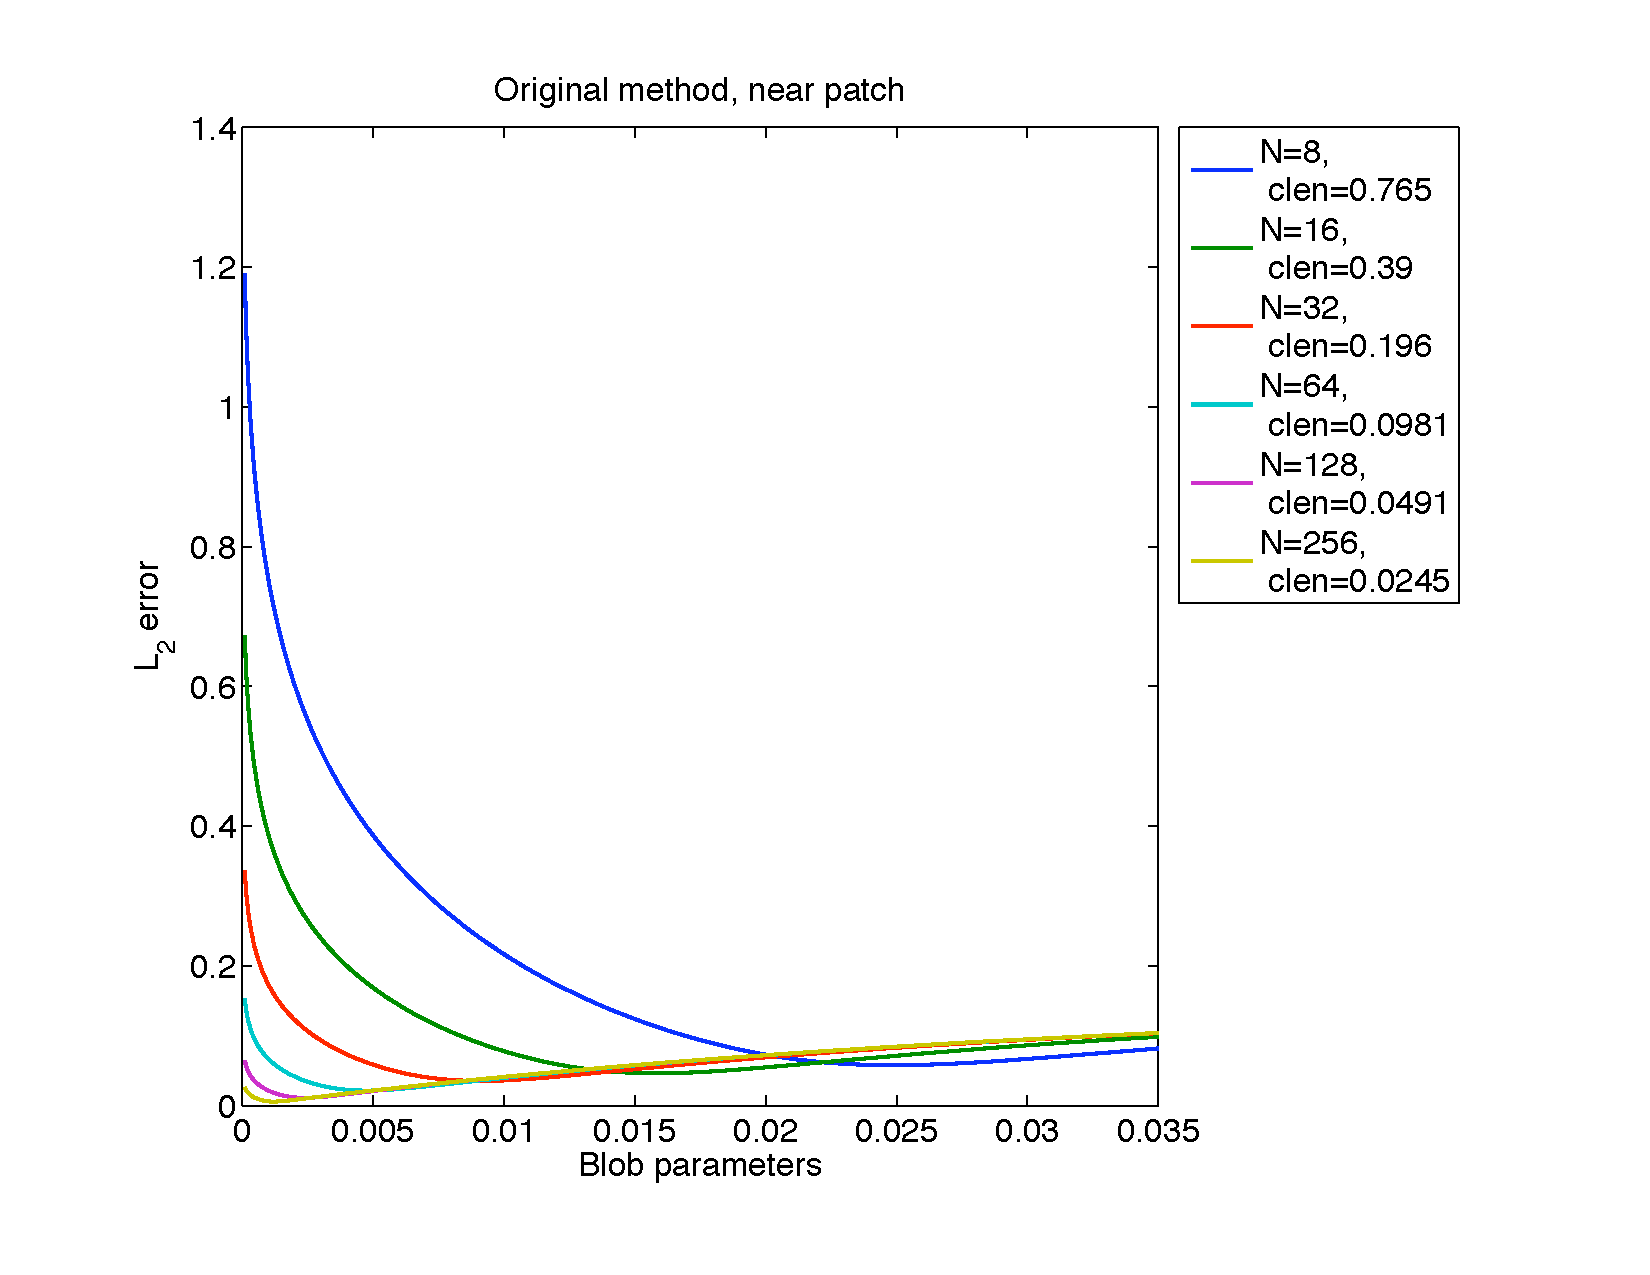
\includegraphics[width=3.75in]{StokesCylTest_farnearpatches_errvsbpnear_origmethod.pdf} & 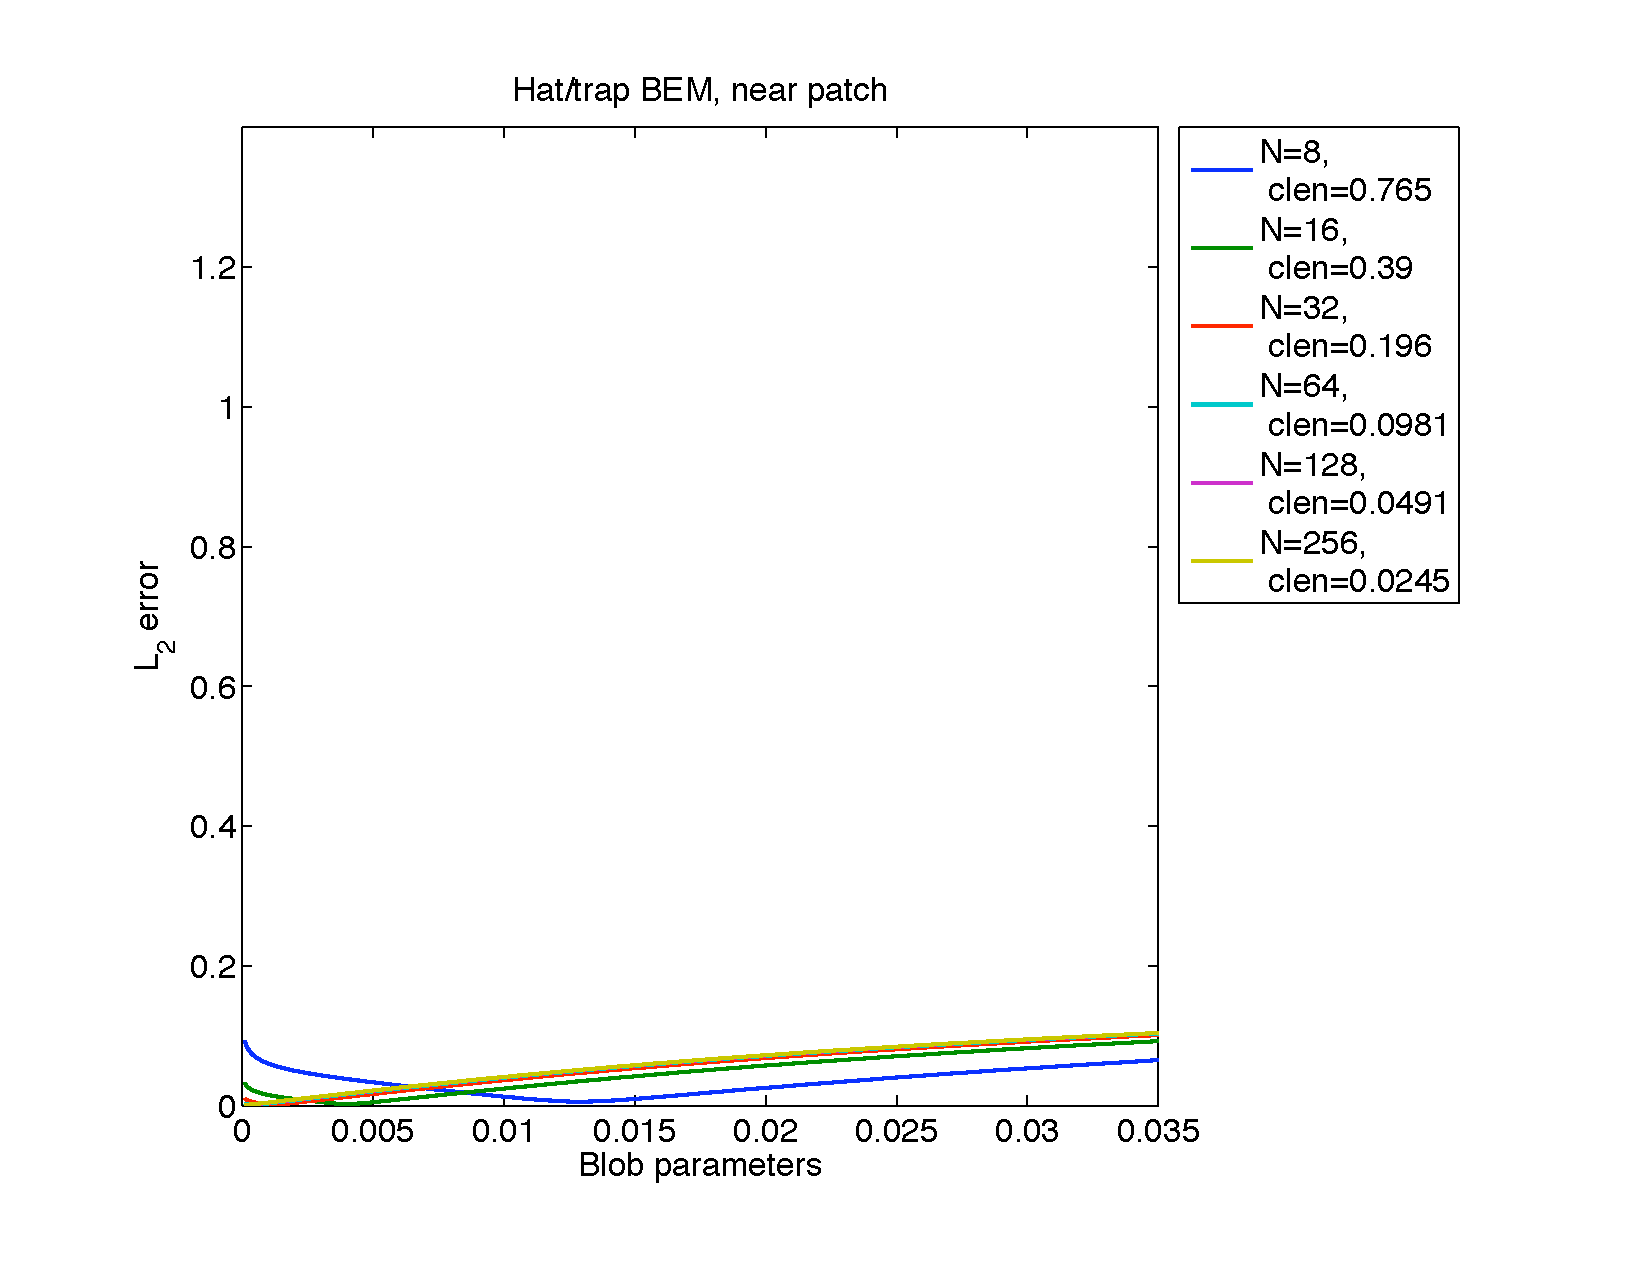
\includegraphics[width=3.75in]{StokesCylTest_farnearpatches_errvsbpnear_hattrap_zoomout.pdf}\\
	A & B \\
	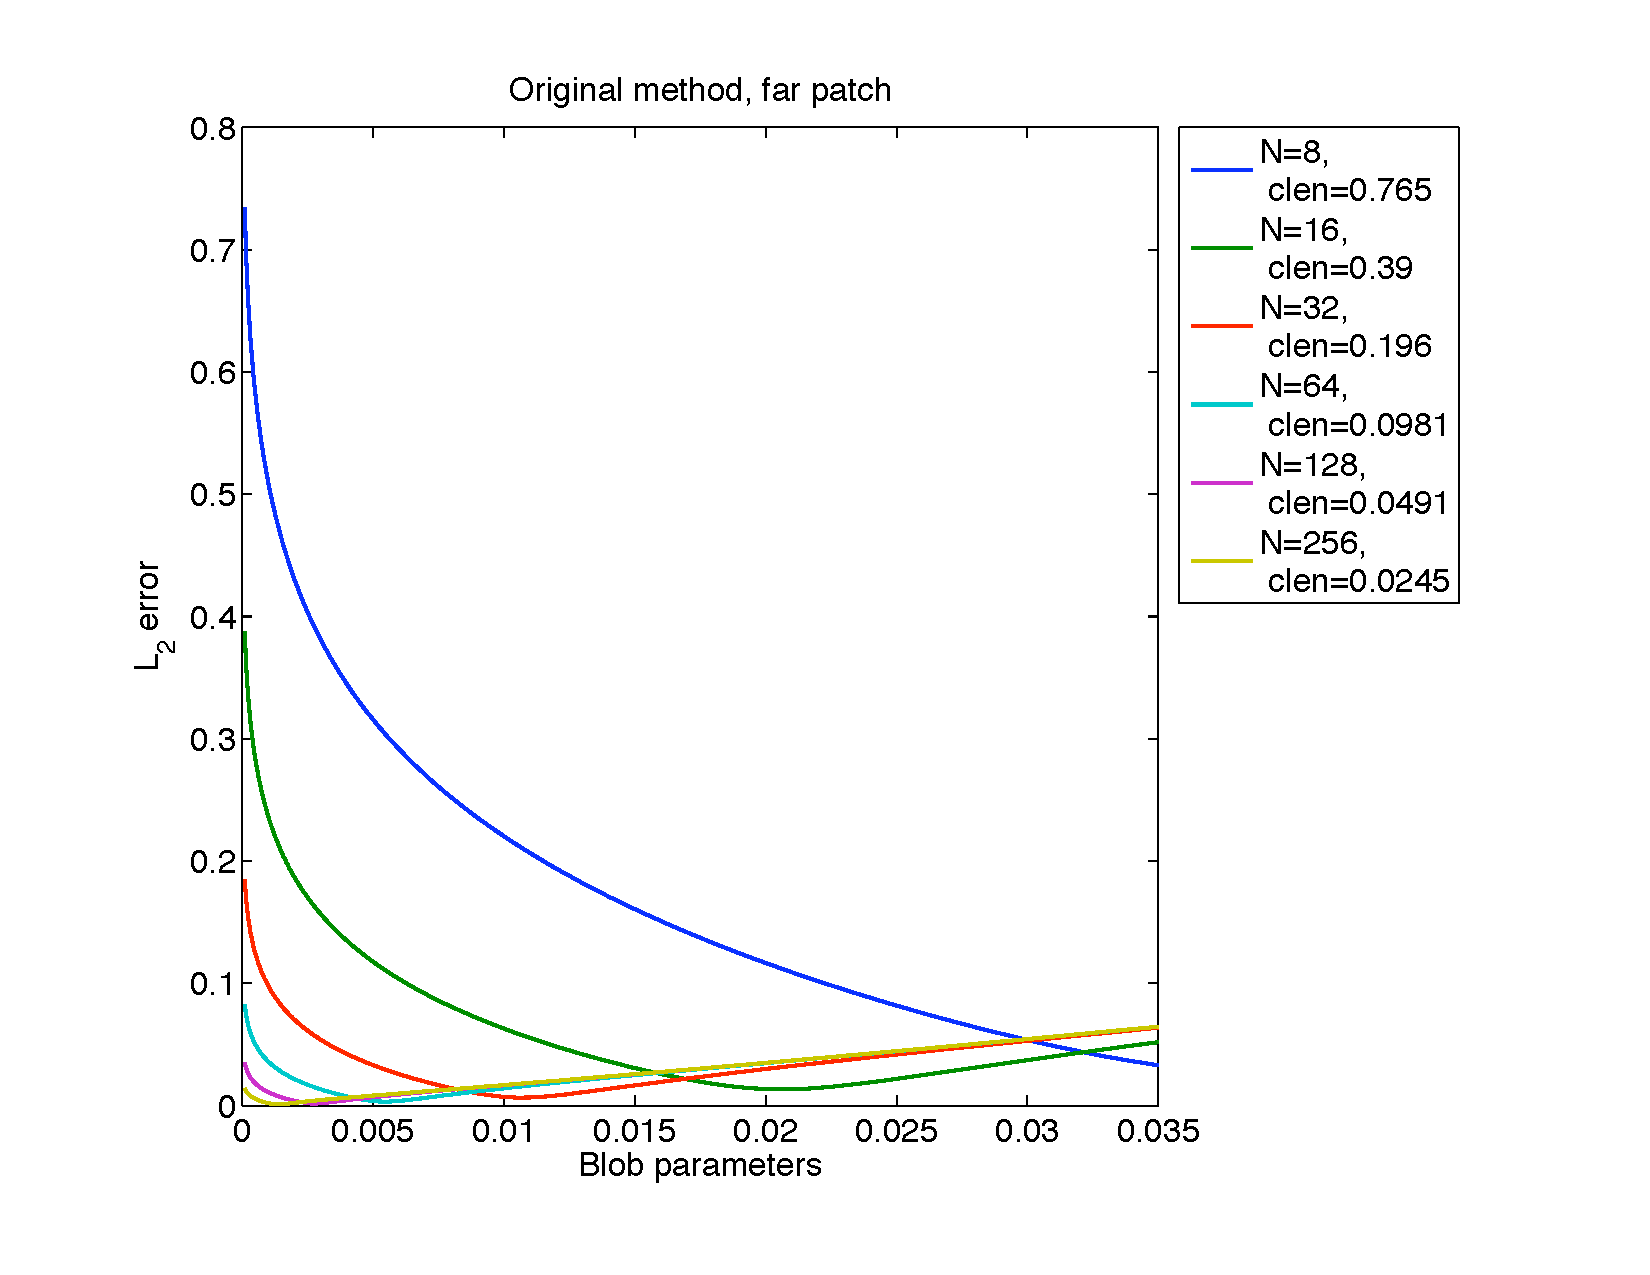
\includegraphics[width=3.75in]{StokesCylTest_farnearpatches_errvsbpfar_origmethod.pdf} & 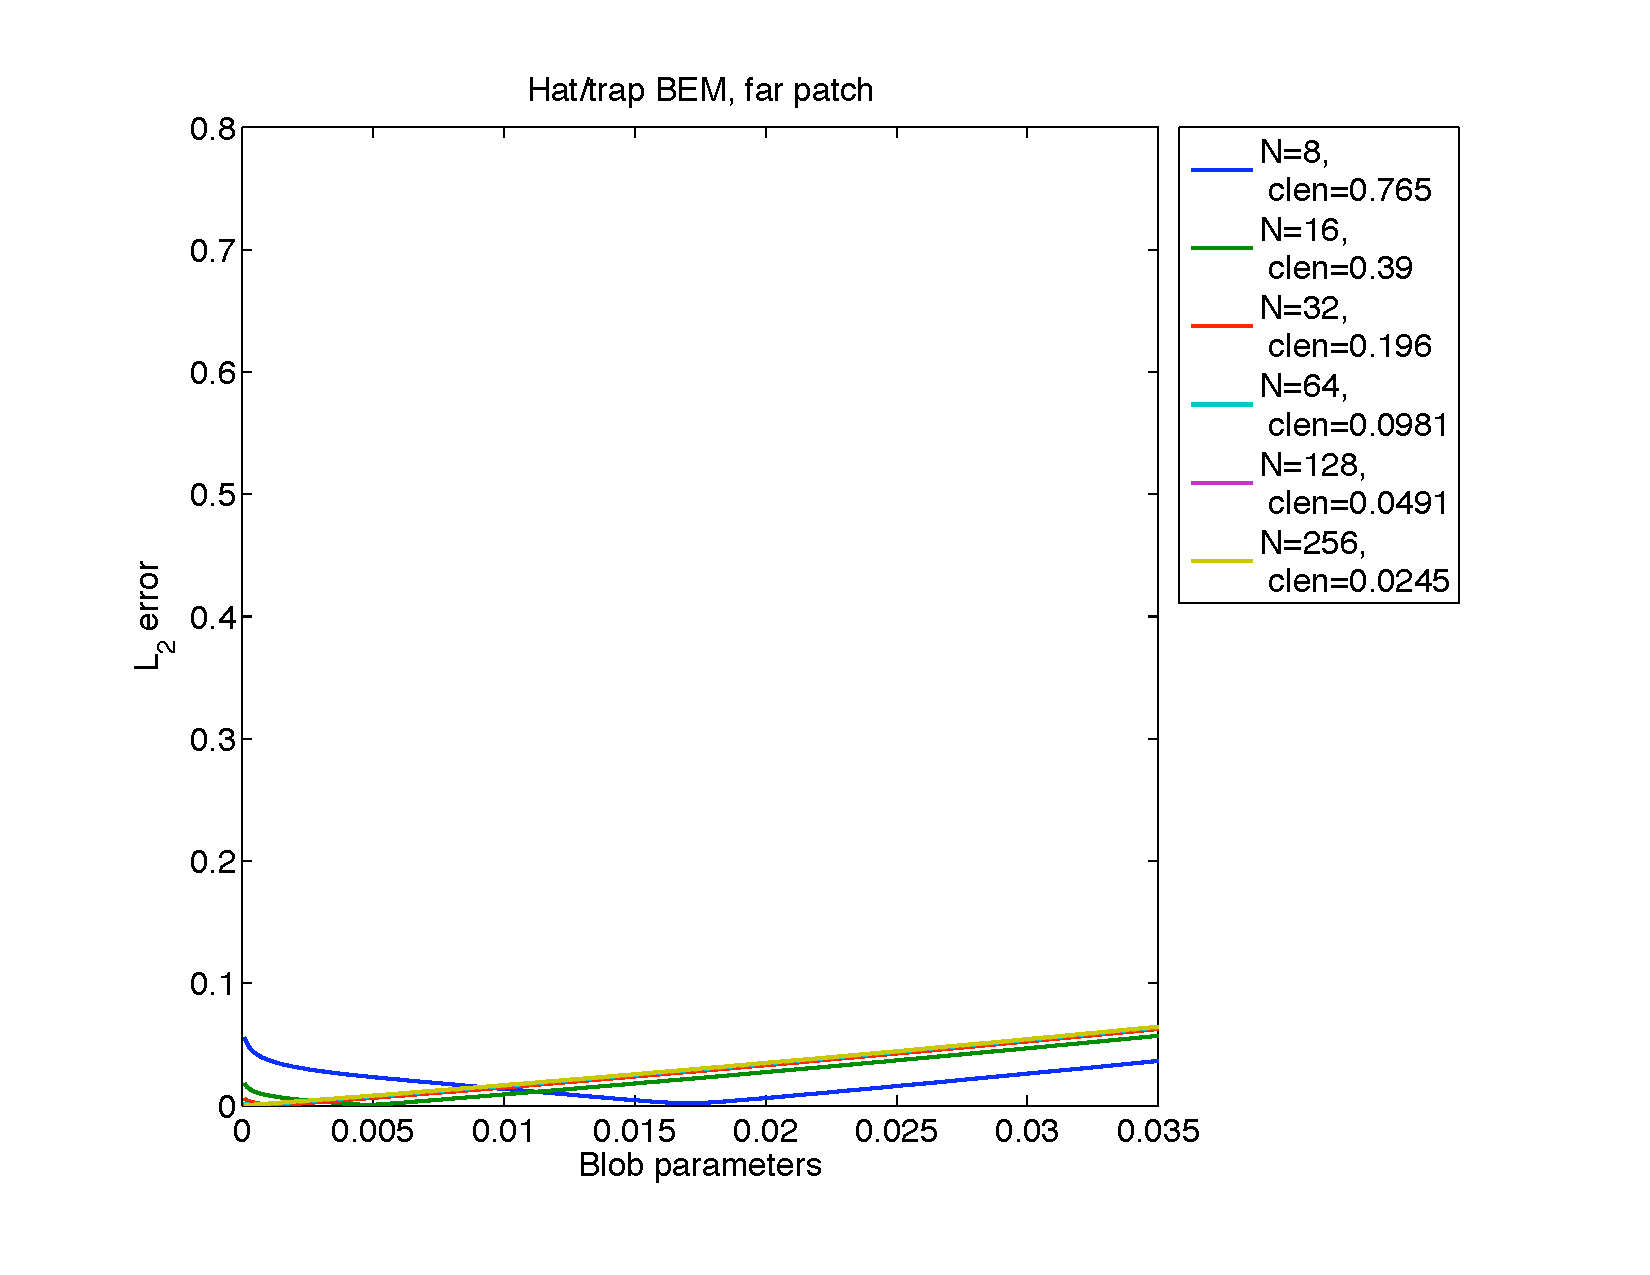
\includegraphics[width=3.75in]{StokesCylTest_farnearpatches_errvsbpfar_hattrap_zoomout.pdf}\\
	C & D	
\end{tabular}
\caption{$L_2$ error versus blob parameter for the near patch (A and B) and the far patch (C and D) using either the original method (A and C) or a BEM using hat functions and the trapezoid rule (B and D).}
\label{errvsbp}
\end{figure}



\begin{figure}[ht]
\begin{tabular}{cc}
	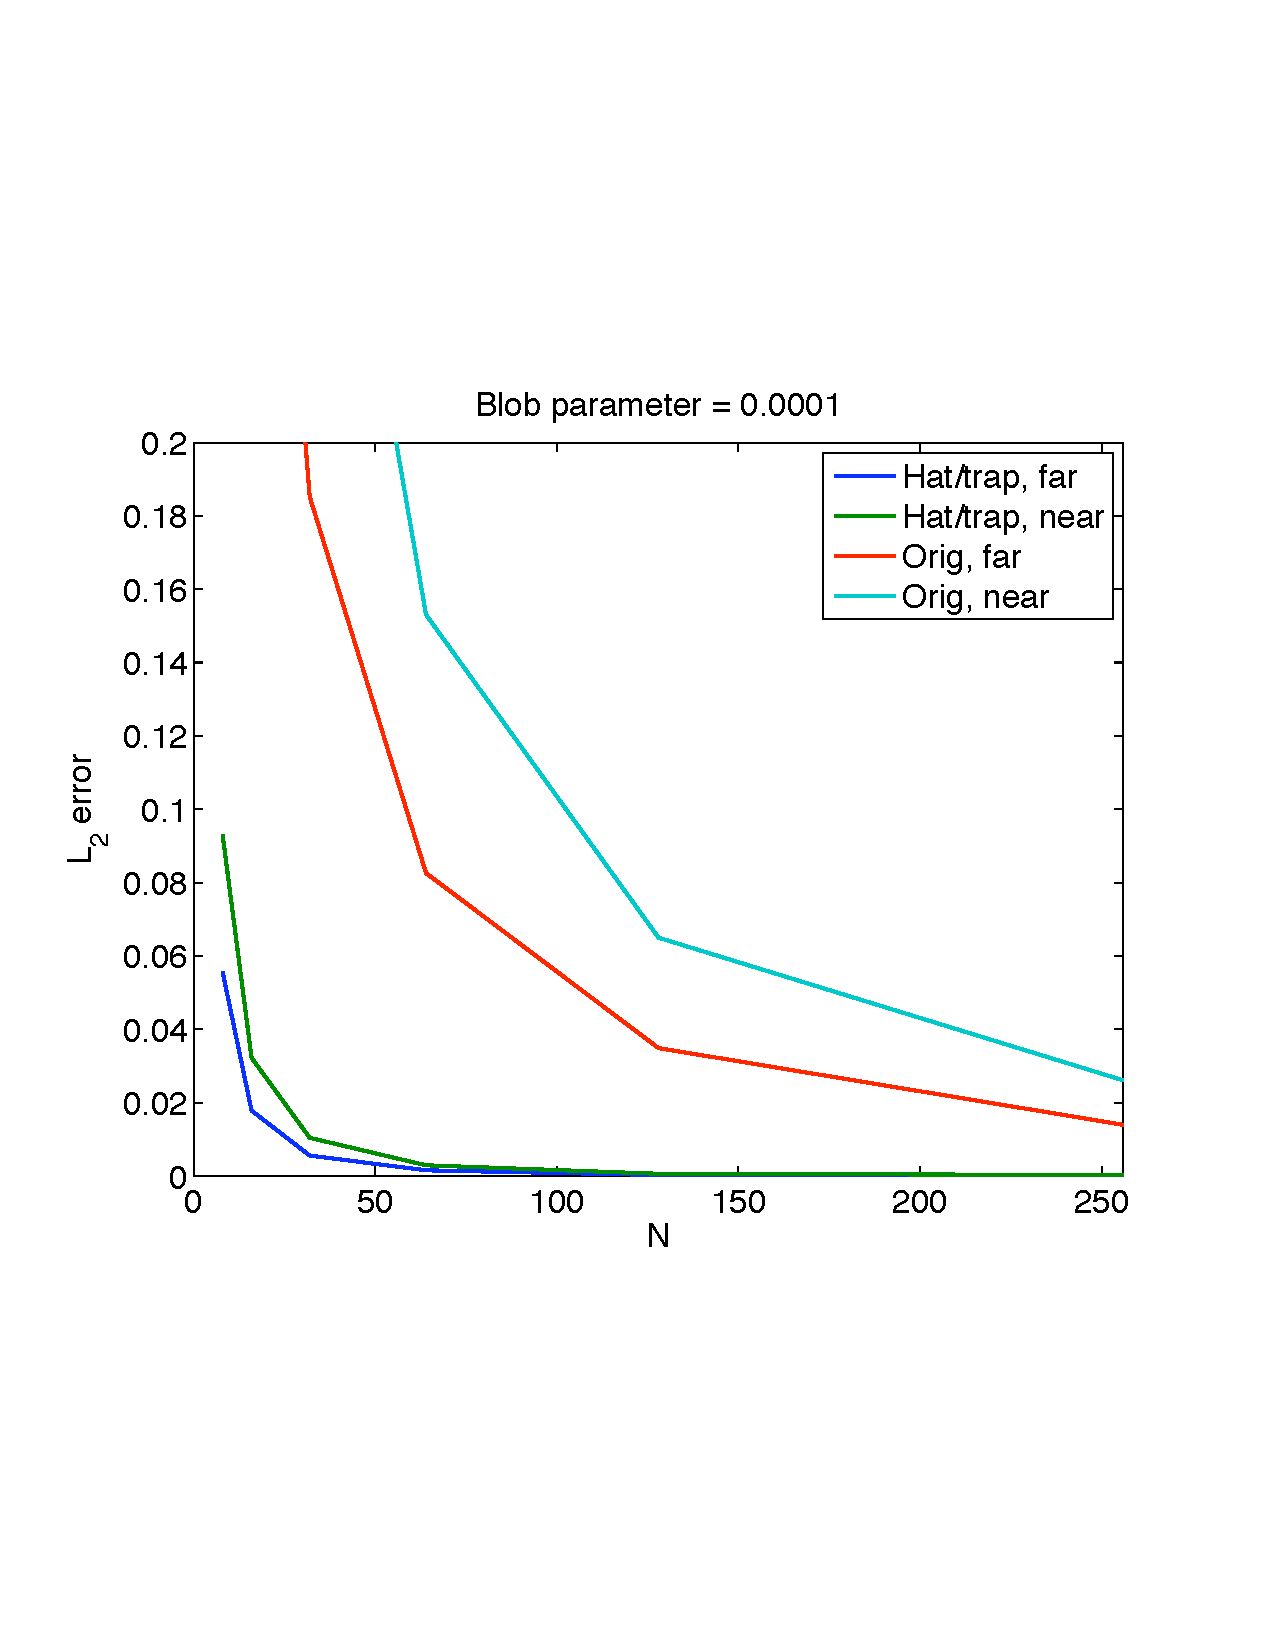
\includegraphics[width=3.75in]{StokesCylTest_farnearpatches_errvsN_blob1e-4.pdf} & 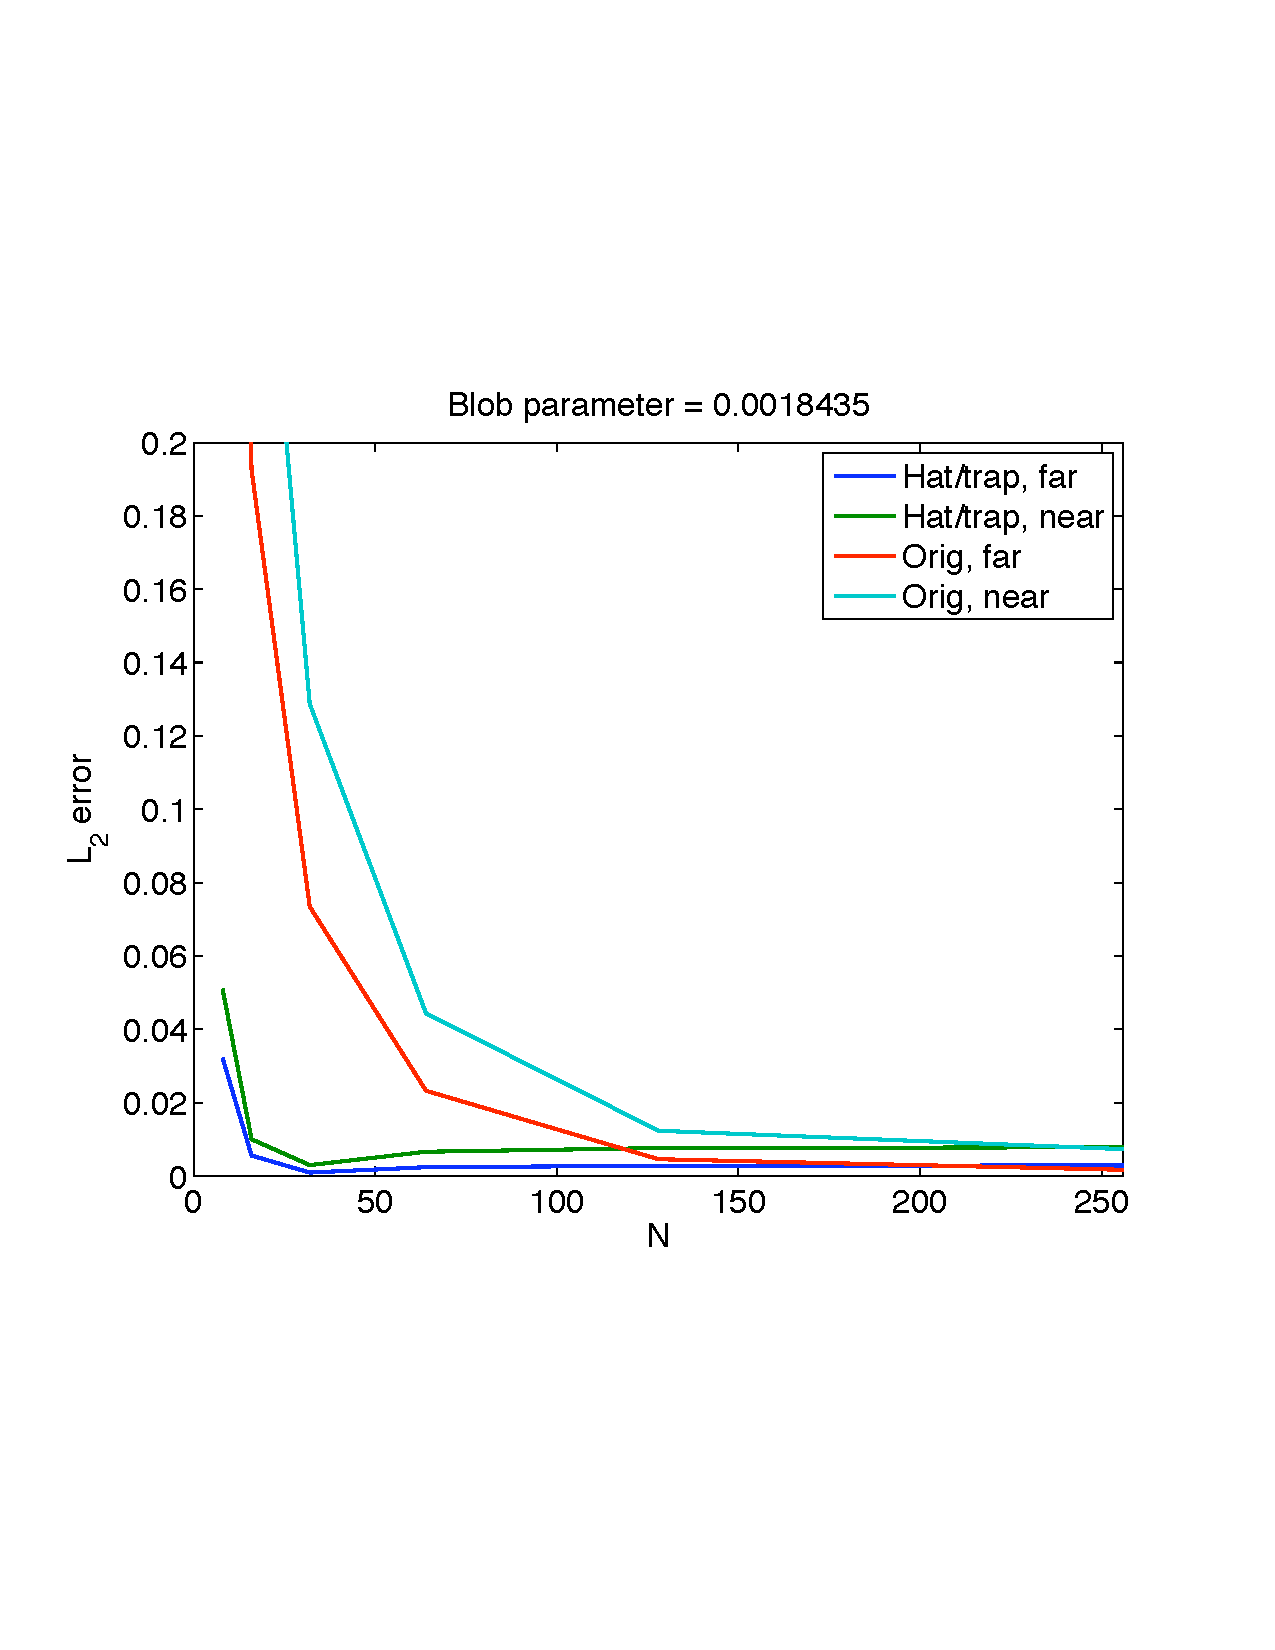
\includegraphics[width=3.75in]{StokesCylTest_farnearpatches_errvsN_blob2e-3.pdf}\\
	A & B \\
	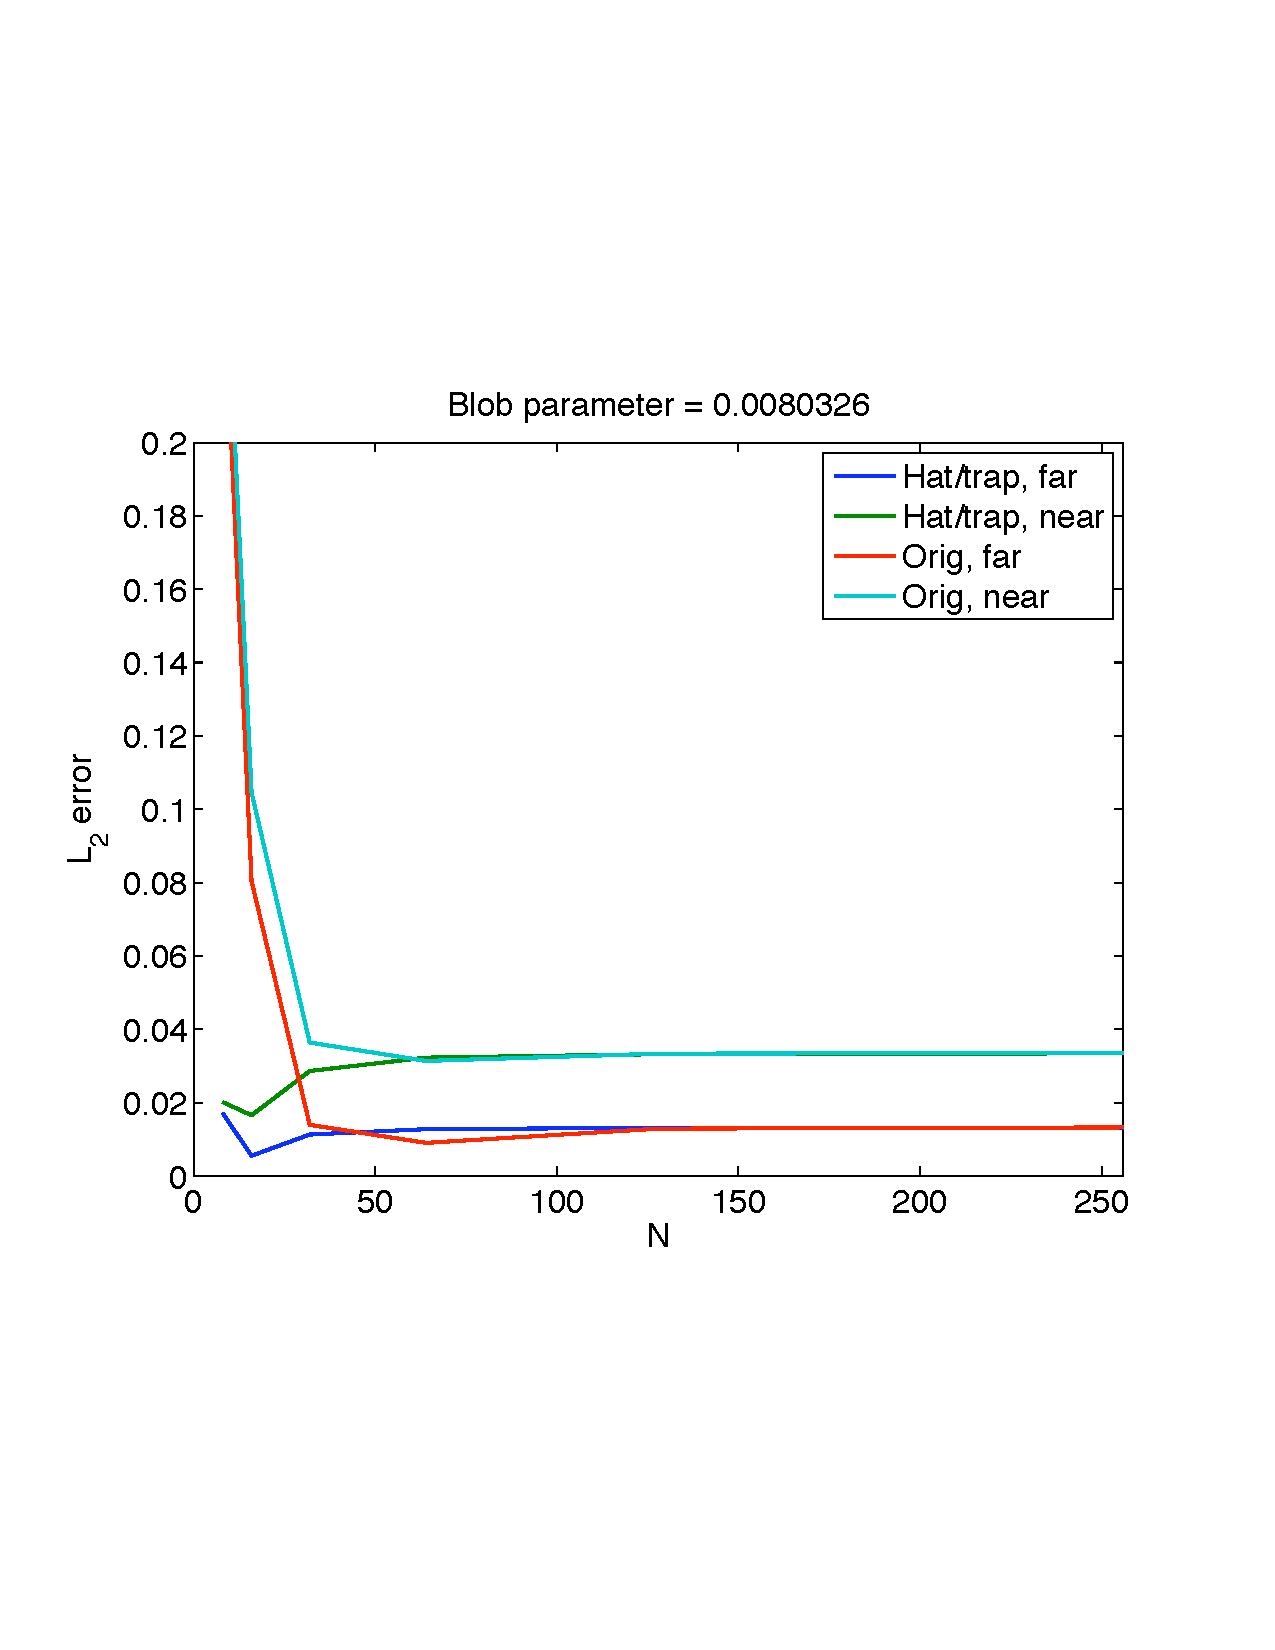
\includegraphics[width=3.75in]{StokesCylTest_farnearpatches_errvsN_blob8e-3.pdf} & 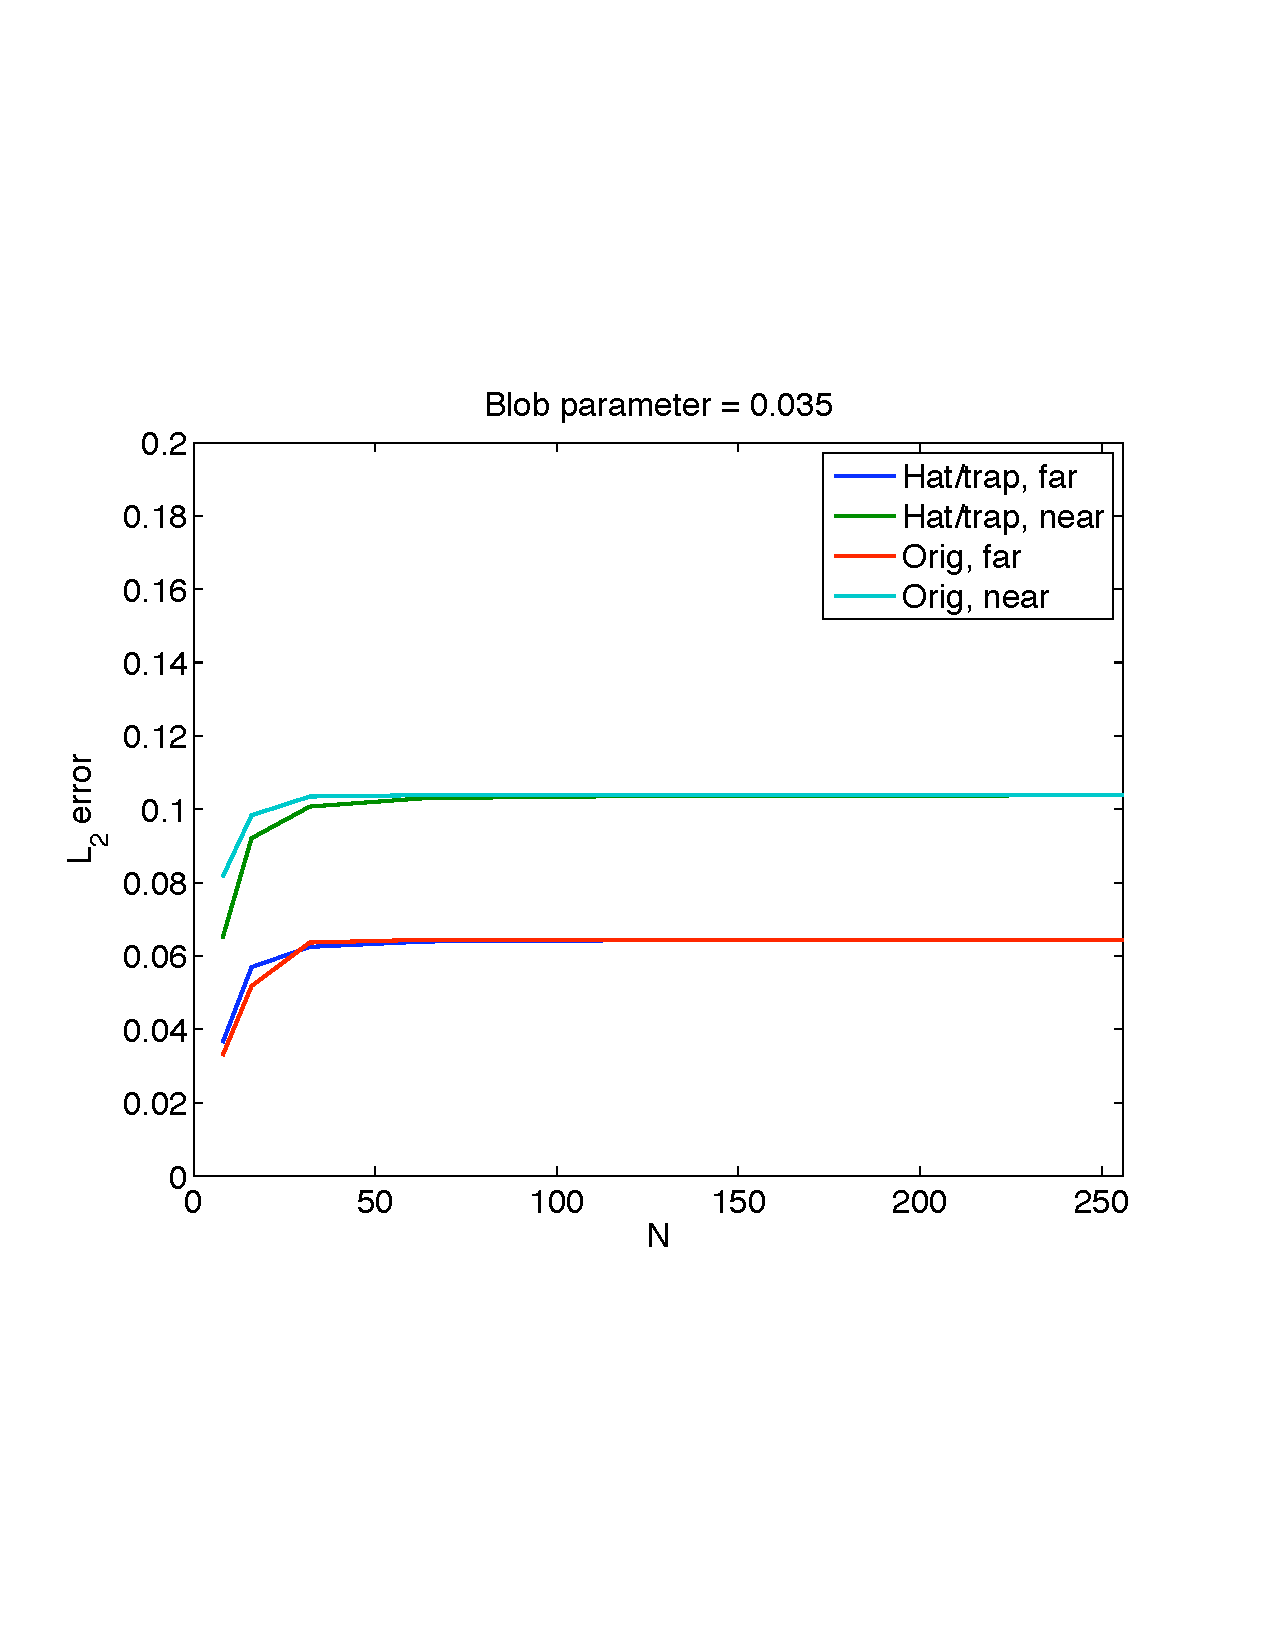
\includegraphics[width=3.75in]{StokesCylTest_farnearpatches_errvsN_blob3e-2.pdf}\\
	C & D	
\end{tabular}
\caption{$L_2$ error versus $N$ for various blob parameters.}
\label{errvsN}
\end{figure}







 
 
 
 





































% Table 2 explores blob parameters from $\ell/2$ to $\ell/64$. In these trials, the basis function is always a hat with $M=10$ and numerical integration is done using the trapezoid rule. Again, the order of convergence is $\ell$. 
% 
% \begin{table}[h]
% 	\begin{centering}
% \begin{tabular}{|c|c|c|c|c|c|c|}
% 	\hline
% 	$N$ & $\ell/2$ & $\ell/4$ & $\ell/8$ & $\ell/16$ & $\ell/32$ & $\ell/64$  \\
% 	\hline
% 				&			&		&			&			&			&			\\
% 	   8 & 1.1731e-02 &  6.5273e-03 &  2.0732e-03 &  6.6497e-03 &  1.1097e-02 &  1.5122e-02  \\
% 	  16 & 1.0170e-02 &  7.1106e-03 &  3.6914e-03 &  1.1501e-03 &  2.3090e-03 &  4.3832e-03  \\
% 	  32 & 8.2617e-03 &  5.5010e-03 &  2.9282e-03 &  1.1945e-03 &  6.4345e-04 &  1.5034e-03  \\
% 	  64 & 5.9626e-03 &  3.4740e-03 &  1.7399e-03 &  7.7297e-04 &  3.5425e-04 &  6.5692e-04  \\
% 	 128 & 3.6181e-03 &  1.8939e-03 &  9.3342e-04 &  4.3919e-04 &  2.0776e-04 &  3.0883e-04  \\
% 	 256 & 1.9302e-03 &  9.6967e-04 &  4.7850e-04 &  2.3094e-04 &  1.1311e-04 &  1.5367e-04  \\
% 	 512 & 9.7898e-04 &  4.8782e-04 &  2.4193e-04 &  1.1839e-04 &  5.9079e-05 &  7.6876e-05  \\
% 				&			&		&			&			&			&			\\
% \hline
% 	$N$ & Err/$\ell$ & Err/$\ell$ & Err/$\ell$ & Err/$\ell$ & Err/$\ell$ & Err/$\ell$  \\
% \hline  
% 			&			&		&			&			&			&			\\
% 	   8 & 1.5328e-02 &  8.5283e-03 &  2.7088e-03 &  8.6883e-03 &  1.4500e-02 &  1.9758e-02  \\
% 	  16 & 2.6064e-02 &  1.8224e-02 &  9.4608e-03 &  2.9476e-03 &  5.9177e-03 &  1.1234e-02  \\
% 	  32 & 4.2144e-02 &  2.8061e-02 &  1.4937e-02 &  6.0933e-03 &  3.2823e-03 &  7.6690e-03  \\
% 	  64 & 6.0759e-02 &  3.5400e-02 &  1.7729e-02 &  7.8766e-03 &  3.6098e-03 &  6.6941e-03  \\
% 	 128 & 7.3715e-02 &  3.8585e-02 &  1.9017e-02 &  8.9480e-03 &  4.2329e-03 &  6.2921e-03  \\
% 	 256 & 7.8646e-02 &  3.9509e-02 &  1.9496e-02 &  9.4096e-03 &  4.6085e-03 &  6.2610e-03  \\
% 	 512 & 7.9775e-02 &  3.9751e-02 &  1.9714e-02 &  9.6472e-03 &  4.8142e-03 &  6.2645e-03  \\
% 				&			&		&			&			&			&			\\
% \hline
% \end{tabular}
% \caption{Errors in BEM on the regularized Stokes cylinder example using hat basis functions with the trapezoid rule. The blob parameter varies from $\ell/2$ to $\ell/64$, where $\ell$ is the chord length. $M$ is fixed at $10$. The values in the upper half of the table are the errors for the point $0.26*(\cos(\pi/6),\sin(\pi/6))$. The values in the lower half of the table are the errors normalized by the chord length.}
% \end{centering}
% \end{table}
% 
% The upper half of Table 2 shows that the ideal choice of blob parameter (in this coarse sampling) is $\ell/N$ for $N=8,\,16,\,32$, and is $\ell/32$ for all higher values of $N$. I was hoping this would shed some light on whether or not there is coupling between the blob parameter and the discretization length scale, but it really doesn't. The blob parameters need to be a fixed set of numbers for all trials in order to assess coupling. The smallest blob in the above table is 
% $2\sin(\pi/512)/64 \approx 1.9175e-4$. The largest blob that I think is worth examination is $2\sin(\pi/8)/4 \approx 1.9134e-1$. An evenly distributed set of parameters in log-10 space is 
% \newline
% [1.9175e\text{-}4,\; 4.1301e\text{-}4,\; 8.8960e\text{-}4,\; 1.9161e\text{-}3, \;4.1272e\text{-}3,\; 8.8897e\text{-}3,\; 1.9148e\text{-}2, \;4.1243e\text{-}2, 8.8833e\text{-}2, \;1.9134e\text{-}1].
% \newline
%  Results for these blob parameters are given in Table 3, with everything else as in Table 2.
% 
% \begin{table}[h]
% 	\begin{centering}
% \begin{tabular}{|c|c|c|c|c|c|c|c|c|c|c|}
% 	\hline
% 	$N$ & 1.918e\text{-}4 & 4.130e\text{-}4 & 8.896e\text{-}4 & 1.916e\text{-}3 & 4.127e\text{-}3 & 8.890e\text{-}3 & 1.915e\text{-}2 & 4.124e\text{-}2  &  8.883e\text{-}2 & 1.913e\text{-}1  \\
% 	\hline
% 	   8 &  3.090e-2 &  2.649e-2 &  2.208e-2 &  1.767e-2 &  1.327e-2 &  8.648e-3 &   3.210e-3 &  5.245e-3  & 1.125e-2 &  1.557e-2 \\
% 	  16 &  1.086e-2 &  8.448e-3 &  6.047e-3 &  3.687e-3 &  1.492e-3 &  2.277e-3 &   5.931e-3 &  9.467e-3  & 1.264e-2 &  1.593e-2 \\
% 	  32 &  3.689e-3 &  2.462e-3 &  1.283e-3 &  6.132e-4 &  1.826e-3 &  4.234e-3 &   7.306e-3 &  1.016e-2  & 1.294e-2 &  1.603e-2 \\
% 	  64 &  1.181e-3 &  6.058e-4 &  3.862e-4 &  1.019e-3 &  2.374e-3 &  4.746e-3 &   7.653e-3 &  1.033e-2  & 1.301e-2 &  1.605e-2 \\
% 	 128 &  3.088e-4 &  2.189e-4 &  5.193e-4 &  1.177e-3 &  2.525e-3 &  4.876e-3 &   7.739e-3 &  1.038e-2  & 1.303e-2 &  1.606e-2 \\
% 	 256 &  1.131e-4 &  2.503e-4 &  5.572e-4 &  1.213e-3 &  2.561e-3 &  4.908e-3 &   7.760e-3 &  1.039e-2  & 1.304e-2 &  1.606e-2 \\
% 	 512 &  1.184e-4 &  2.608e-4 &  5.665e-4 &  1.222e-3 &  2.570e-3 &  4.916e-3 &   7.765e-3 &  1.039e-2  & 1.304e-2 &  1.606e-2 \\
% \hline
% \end{tabular}
% \caption{Errors in BEM on the regularized Stokes cylinder example using hat basis functions with the trapezoid rule. The blob parameter varies from 1.9175e-4 to 1.9134e-1. $M$ is fixed at $10$. The values in the table are the errors for the point $0.26*(\cos(\pi/6),\sin(\pi/6))$. }
% \end{centering}
% \end{table}

\end{document}

  
  
  
  
  
  
  
  
  
  
  
  


   
   
   
   
   
   
   























